\subsection{Elementary particles in the Standard Model}
\label{elementaryparticles}

The elementary particles in SM can be classified into 3 class: \textit{fermions, gauge bosons and the Higgs boson} as shown in Figure~\ref{fig:eleP-1}.
\begin{figure}[!htb]
  \centering
  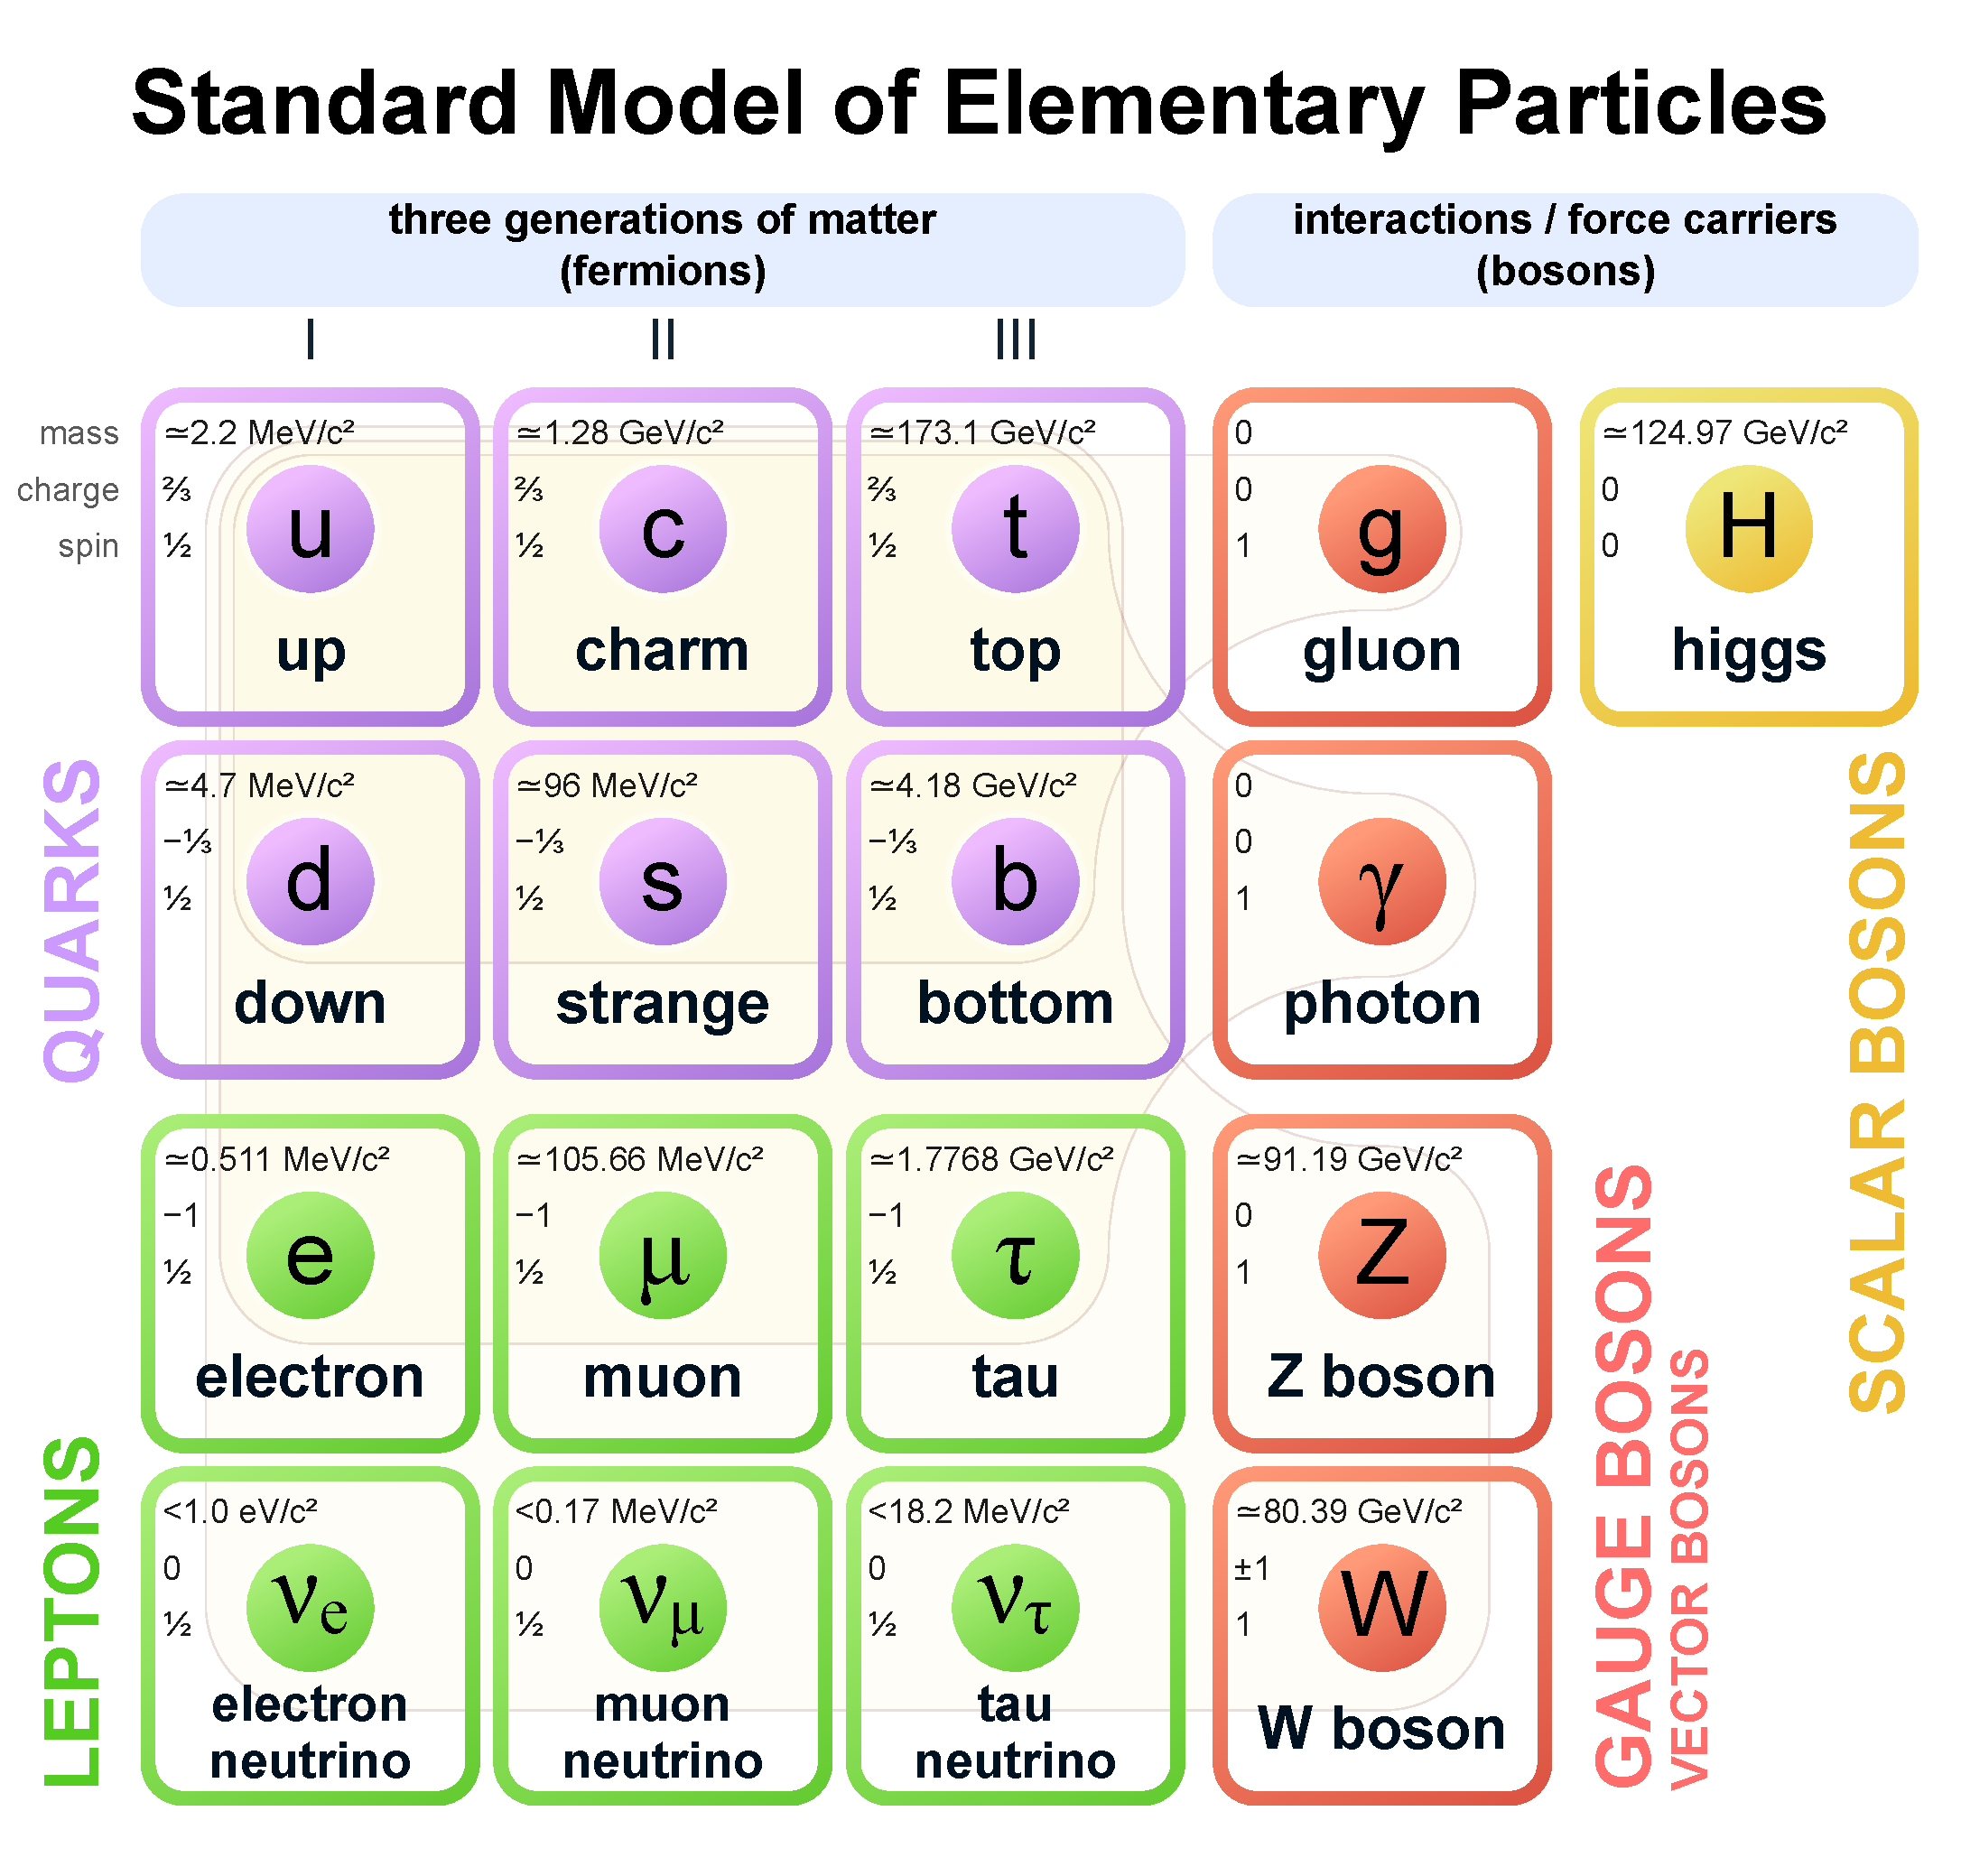
\includegraphics[width=0.48\textwidth]{figures/Theory/Standard_Model_of_Elementary_Particles.pdf}
  \caption{The elementary particles of the Standard Model.}
  \label{fig:eleP-1}
\end{figure}

\textbf{Fermions}
The Standard Model includes 12 elementary particles of spin-$\frac{1}{2}$ obeying the Fermy-Dirac statistics, known as fermions. 
They are classified into two types: \textit{leptons and quarks} according to the their interctions.
The \textit{leptons} include three generations: electron ($e$) and electron neutrino ($\nu_{e}$); 
muon ($\mu$) and muon neutrino ($\nu_{\mu}$); tau ($\tau$) and tau neutrino ($\nu_{\tau}$).
The $e, \mu~and~\tau$ carry electric charge of -1 and three neutrinos are electrically neutral. 
All the leptons can participate in electroweak interactions.
Also there are three generations of \textit{quarks}: up ($u$) and down ($d$); charm ($c$) and strange ($s$); top ($t$) and bottom ($b$).
The defining property of the quarks is that they carry color charge (while leptons don't), and hence interact via the strong interaction, 
leting them be strongly bound from one to another, forming color-neutral composite 
particles (hadrons) containing either a quark and an antiquark (mesons) or three quarks (baryons).
In the meantime, u, c and t-quark carry electric charge of 2/3, and d, s and b-quark carry electric charge of -1/3. 
Hence they interact via all three interactions described in SM.
Each fermion also has a corresponding antiparticles.

\textbf{Gauge bosons}
act as force carriers that mediate the strong, weak, and electromagnetic interactions in SM.
They are spin-1 particles obeying the Bose-Einstein statistics. 
There are three types of gauge bosons:
\begin{itemize}
  \item The eight massless \textit{gluons} mediate the strong interactions between color charged particles (the quarks).
  \item The massless \textit{photons} mediate the electromagnetic force between electrically charged particles.
  \item The $W^{+}, W^{-} and Z$ bosons mediate the weak interactions between particles of different flavors (all quarks and leptons). All these three bosons are masive, the $W^{\pm}$ carries an electric charge of $+1$ and $−1$ and couples to the electromagnetic interaction. Z boson is electrically neutral.
\end{itemize}
Figure~\ref{fig:eleP-2} shows the Feynman diagrams of corresponding interactions in SM.
\begin{figure}[!htb]
  \centering
  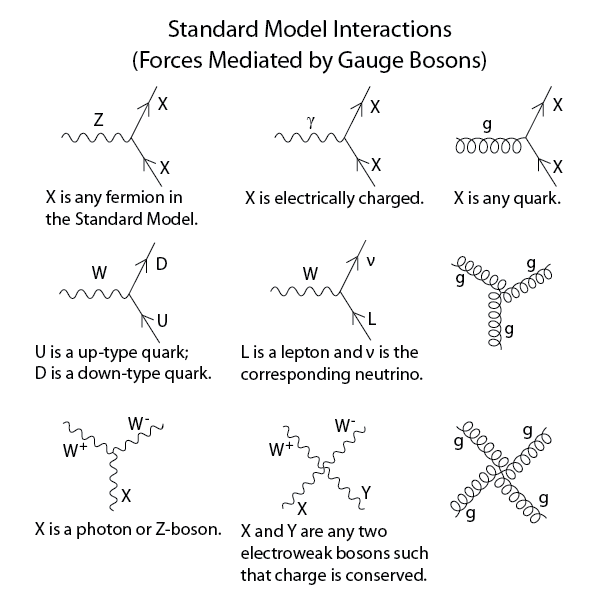
\includegraphics[width=0.48\textwidth]{figures/Theory/Standard_Model_Feynman_Diagram_Vertices.png}
  \caption{The Feyman diagrams of interactions that form the basis of the standard model.}
  \label{fig:eleP-2}
\end{figure}

\textbf{Higgs boson}
is a masive scaler elementary particle with spin-0. 
It plays a unique role in the SM by explainning the origin of masses of massive gauge bosons ($W^{\pm} and Z$) and fermions. 
And it is the last discovered particle in SM.
